\subchapter{Configuring pin muxing}
{Objective: learn how to declare and use a muxing state.}

\section{Goals}

As part of the previous lab, we enabled an I2C controller and described
a device plugged on the bus. In this lab we will cover how to ensure a
proper communication between the two and be able to declare and use
pinctrl settings.

\section{Setup}

Continue using the \code{bootlin-labs} branch in the
\code{~/linux-kernel-labs/src/linux} directory.

\section{Probing the different busses}

The STM32MP157D-DK1 device tree already correctly configures the pinmuxing state
for the I2C5 bus. Before proceeding with this lab, we ask you to delete this
pinmuxing configuration by adding three lines in your custom device tree:

\begin{verbatim}
&i2c5 {
+       /delete-property/ pinctrl-0;
+       /delete-property/ pinctrl-1;
+       /delete-property/ pinctrl-names;
\end{verbatim}

Reboot your board with these changes.
Now, let's use \code{i2cdetect}'s capability to probe a bus for
devices. The I2C bus has no real discovery capability, but yet, the tool
exploits a feature of the specification: when the master talks to a
device, it starts by sending the target address on the bus and expects
it to be acked by the relevant device. Iterating through all the
possible addresses without sending anything after the address byte,
looking for the presence of an Ack is what uses the tool to probe the
devices. That is also why we get a warning when using it.

Let's start by probing the bus associated to \code{i2c-2}:

\begin{bashinput}
# i2cdetect -r 2
i2cdetect: WARNING! This program can confuse your I2C bus
Continue? [y/N] y
     0  1  2  3  4  5  6  7  8  9  a  b  c  d  e  f
00:          -- -- -- -- -- -- -- -- -- -- -- -- -- 
10: -- -- -- -- -- -- -- -- -- -- -- -- -- -- -- -- 
20: -- -- -- -- -- -- -- -- 28 -- -- -- -- -- -- -- 
30: -- -- -- UU -- -- -- -- -- -- -- -- -- -- -- -- 
40: -- -- -- -- -- -- -- -- -- -- -- -- -- -- -- -- 
50: -- -- -- -- -- -- -- -- -- -- -- -- -- -- -- -- 
60: -- -- -- -- -- -- -- -- -- -- -- -- -- -- -- -- 
70: -- -- -- -- -- -- -- --                         
\end{bashinput}

We can see two devices on this internal bus:
\begin{itemize}
\item One at address \code{0x33}, indicated by \code{UU},
      which means that there is a kernel driver actively
      driving this device.
\item Another one at address \code{0x28}.
      We just know that they are currently not bound to a kernel driver.
\end{itemize}

Now try to probe I2C5 with \code{i2cdetect -r 1}.

You will see that the command will fail to connect to
the bus. That's because the corresponding signals are
not exposed yet to the outside connectors through pin muxing.

\section{Find pin muxing configuration information for i2c5}

As you found in the previous lab, we now managed to have our nunchuk device
enumerated on the \code{i2c5} bus.

However, to access the bus data and clock signals, we need to configure the
pin muxing of the SoC.

If you open the STM32MP157 user manual and go to sheet 28, you’ll see that the
\code{I2C5_SDA} and \code{I2C5_SCL} signals are routed to pins
PA12 and PA11 on the STM32MP157 SoC.

Now open the STM32MP157A/D datasheet (not the reference manual!) and go to
Table 8. Alternate functions AF0 to AF7. Search for pins PA11 and PA12 in
this table. Once you’ve found pins PA11 and PA12, you’ll see that pin mux
number 4 corresponds to the \code{I2C5_SDA} and \code{I2C5_SCL} signals.

In the STM32MP157 reference manual, you’ll find the addresses of the pad
configuration registers for these pins. Register 0x50002024 configures PA12 and
PA11.

We now know which register we can write to enable i2c5 signals

\section{Multiplexing the I2C controller outputs correctly}

Now that we know the register offsets, let's try to understand
how they are used in existing code. For example, open the
the Device Tree describing the pinctrl for the STM32MP15XX boards
(\kfile{arch/arm/boot/dts/st/stm32mp15-pinctrl.dtsi}).
Look for \code{i2c5_pins_a}, and you will see how offsets are declared and
what values they are given:

\begin{verbatim}
i2c5_pins_a: i2c5-0 {
        pins {
                pinmux = <STM32_PINMUX('A', 11, AF4)>, /* I2C5_SCL */
                         <STM32_PINMUX('A', 12, AF4)>; /* I2C5_SDA */
                         bias-disable;
                         drive-open-drain;
                         slew-rate = <0>;
        };
};
\end{verbatim}

As expected, we could confirm the pin muxing usage described earlier.

Now that pin muxing settings have been explained, you can remove the three
delete-property lines that you added to your custom device tree.
Rebuild and update your DTB, then reboot the board. You should now be able to
probe your bus:

\begin{bashinput}
# i2cdetect -r 1
i2cdetect: WARNING! This program can confuse your I2C bus
Continue? [y/N] y
     0  1  2  3  4  5  6  7  8  9  a  b  c  d  e  f
00:          -- -- -- -- -- -- -- -- -- -- -- -- --
10: -- -- -- -- -- -- -- -- -- -- -- -- -- -- -- --
20: -- -- -- -- -- -- -- -- -- -- -- -- -- -- -- --
30: -- -- -- -- -- -- -- -- -- -- -- -- -- -- -- --
40: -- -- -- -- -- -- -- -- -- -- -- -- -- -- -- --
50: -- -- -- -- -- -- -- -- -- -- -- -- -- -- -- --
60: -- -- -- -- -- -- -- -- -- -- -- -- -- -- -- --
70: -- -- -- -- -- -- -- --
\end{bashinput}

No devices are detected, because we did not wire the nunchuk yet.

\subsection{Wiring the I2C device}

Let's connect the Nunchuk provided by your instructor
to the I2C1 bus on the board, using breadboard wires:

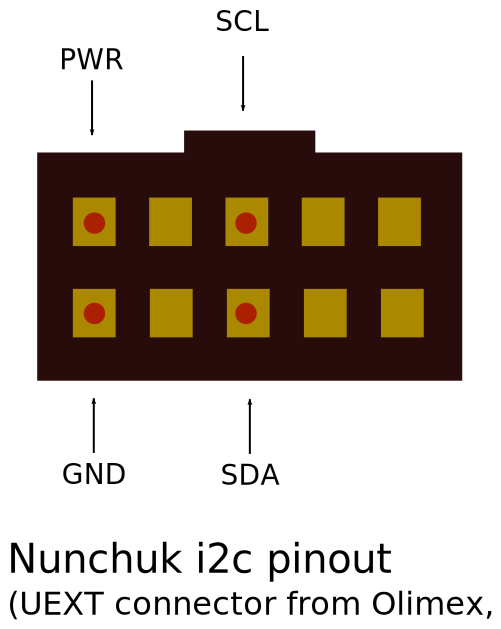
\includegraphics[width=0.3\textwidth]{common/nunchuk-pinout.pdf}
\includegraphics[width=0.7\textwidth]{labs/kernel-i2c-multiplexing-stm32mp1/stm32mp1-connect-nunchuk.jpg}

\begin{itemize}
\item Connect the Nunchuk PWR pin to pin 1 (3V3) of GPIO connector CN2
\item Connect the Nunchuk GND pin to pin 6 (GND) of GPIO connector CN2
\item Connect the Nunchuk SCL pin to pin 5 of GPIO connector CN2
\item Connect the Nunchuk SDA pin to pin 3 of GPIO connector CN2
\end{itemize}

If you didn't do any mistake, your new device should be detected at
address \code{0x52}:

\begin{bashinput}
# i2cdetect -r 1
i2cdetect: WARNING! This program can confuse your I2C bus
Continue? [y/N] y
     0  1  2  3  4  5  6  7  8  9  a  b  c  d  e  f
00:          -- -- -- -- -- -- -- -- -- -- -- -- --
10: -- -- -- -- -- -- -- -- -- -- -- -- -- -- -- --
20: -- -- -- -- -- -- -- -- -- -- -- -- -- -- -- --
30: -- -- -- -- -- -- -- -- -- -- -- -- -- -- -- --
40: -- -- -- -- -- -- -- -- -- -- -- -- -- -- -- --
50: -- -- 52 -- -- -- -- -- -- -- -- -- -- -- -- --
60: -- -- -- -- -- -- -- -- -- -- -- -- -- -- -- --
70: -- -- -- -- -- -- -- --
\end{bashinput}

We will later compile an out-of-tree kernel module to support this device.
